\documentclass{article}
\usepackage{fontspec}
\setmainfont{Times New Roman}
\usepackage{geometry}
\usepackage{CTEX}
\geometry{papersize={21cm,29.7cm}}
\geometry{left=3.18cm,right=3.18cm,top=2.54cm,bottom=2.54cm}
\usepackage{fancyhdr}
\usepackage{amsmath}
\pagestyle{fancy}
\lhead{学号:202000460020}
\rhead{姓名:苏博南}
\cfoot{\thepage}
\renewcommand{\headrulewidth}{0.4pt}
\renewcommand{\headwidth}{\textwidth}
\usepackage{tikz}
\usetikzlibrary{automata, positioning, arrows}
\usepackage{listings}
\usepackage{float}
\lstset{
	basicstyle=\small\ttfamily,	% 基本样式
		keywordstyle=\color{blue}, % 关键词样式
		commentstyle=\color{gray!50!black!50},   	% 注释样式
		stringstyle=\rmfamily\slshape\color{red}, 	% 字符串样式
	backgroundcolor=\color{gray!0},     % 代码块背景颜色
	frame=leftline,						% 代码框形状
	framerule=12pt,%
		rulecolor=\color{gray!0},      % 代码框颜色
	numbers=left,				% 左侧显示行号往左靠, 还可以为right ,或none,即不加行号
		numberstyle=\footnotesize\itshape,	% 行号的样式
		firstnumber=1,
		stepnumber=1,                  	% 若设置为2,则显示行号为1,3,5
		numbersep=7pt,               	% 行号与代码之间的间距
	aboveskip=.25em, 			% 代码块边框
	showspaces=false,               	% 显示添加特定下划线的空格
	showstringspaces=false,         	% 不显示代码字符串中间的空格标记
	keepspaces=true, 					
	showtabs=false,                 	% 在字符串中显示制表符
	tabsize=2,                     		% 默认缩进2个字符
	captionpos=b,                   	% 将标题位置设置为底部
	flexiblecolumns=true, 			%
	breaklines=true,                	% 设置自动断行
	breakatwhitespace=false,        	% 设置自动中断是否只发生在空格处
	breakautoindent=true,			%
	breakindent=1em, 			%
	title=\lstname,				%
	escapeinside=``,  			% 在``里显示中文
	xleftmargin=1em,  xrightmargin=1em,     % 设定listing左右的空白
	aboveskip=1ex, belowskip=1ex,
	framextopmargin=1pt, framexbottommargin=1pt,
        abovecaptionskip=-2pt,belowcaptionskip=3pt,
	% 设定中文冲突,断行,列模式,数学环境输入,listing数字的样式
	extendedchars=false, columns=flexible, mathescape=true,
	texcl=true,
	fontadjust
}%
\newtheorem{question}{题目}  
\lstset{
	basicstyle=\small\ttfamily,	% 基本样式
		keywordstyle=\color{blue}, % 关键词样式
		commentstyle=\color{gray!50!black!50},   	% 注释样式
		stringstyle=\rmfamily\slshape\color{red}, 	% 字符串样式
	backgroundcolor=\color{gray!0},     % 代码块背景颜色
	frame=leftline,						% 代码框形状
	framerule=12pt,%
		rulecolor=\color{gray!0},      % 代码框颜色
	numbers=left,				% 左侧显示行号往左靠, 还可以为right ,或none,即不加行号
		numberstyle=\footnotesize\itshape,	% 行号的样式
		firstnumber=1,
		stepnumber=1,                  	% 若设置为2,则显示行号为1,3,5
		numbersep=7pt,               	% 行号与代码之间的间距
	aboveskip=.25em, 			% 代码块边框
	showspaces=false,               	% 显示添加特定下划线的空格
	showstringspaces=false,         	% 不显示代码字符串中间的空格标记
	keepspaces=true, 					
	showtabs=false,                 	% 在字符串中显示制表符
	tabsize=2,                     		% 默认缩进2个字符
	captionpos=b,                   	% 将标题位置设置为底部
	flexiblecolumns=true, 			%
	breaklines=true,                	% 设置自动断行
	breakatwhitespace=false,        	% 设置自动中断是否只发生在空格处
	breakautoindent=true,			%
	breakindent=1em, 			%
	title=\lstname,				%
	escapeinside=``,  			% 在``里显示中文
	xleftmargin=1em,  xrightmargin=1em,     % 设定listing左右的空白
	aboveskip=1ex, belowskip=1ex,
	framextopmargin=1pt, framexbottommargin=1pt,
        abovecaptionskip=-2pt,belowcaptionskip=3pt,
	% 设定中文冲突,断行,列模式,数学环境输入,listing数字的样式
	extendedchars=false, columns=flexible, mathescape=true,
	texcl=true,
	fontadjust
}%

\begin{document}

\begin{center}
    \huge{机器学习课程实验十}\\
    \large{\today \quad 苏博南\quad 202000460020}
\end{center}
\section{Linear Support Vector Machine(SVM)}
\subsection{理论推导}

对于一个样本点$\textbf{x}_i$,和一个超平面$\textbf{w}^T\textbf{x}+b=0$,我们定义点到平面的距离为:
\begin{equation}
	distance=\frac{|\textbf{w}^T\textbf{x}_i+b|}{||\textbf{w}||}
\end{equation}

那么对于一个可线性二分类的数据集,我们不仅希望得到一个超平面划分它,还希望两边正负数据离超平面的\textbf{最短距离尽量大}。
即我们希望:
\begin{equation}
	\begin{cases}
		\frac{|\textbf{w}^T\textbf{x}_i+b|}{||\textbf{w}||}\geq\frac{m}{2} & y_i=1\\
		\frac{|\textbf{w}^T\textbf{x}_i+b|}{||\textbf{w}||}\leq-\frac{m}{2} & y_i=-1
	\end{cases}
\end{equation}

其中,$\frac{m}{2}$就是正,负类样本点距离超平面的最小距离:
\begin{figure}[H]
	\centering
	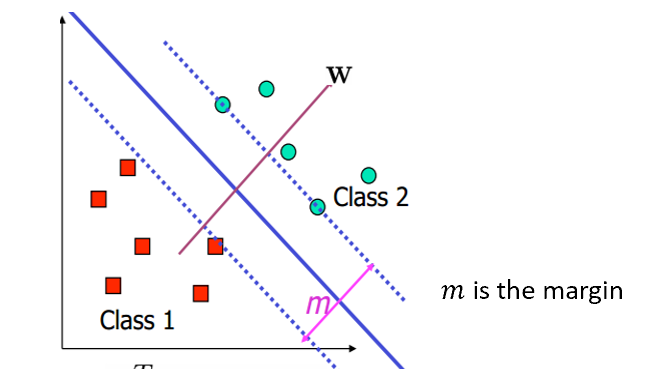
\includegraphics[width=0.6\linewidth]{4.png}
\end{figure}

然后处理下,我们可以记$\textbf{w}'=\frac{2\textbf{w}}{||\textbf{w}||m},b'=\frac{2b}{||\textbf{w}||m}$,则有:
\begin{equation}
	\begin{cases}
		\textbf{w}'^T\textbf{x}_i+b'\geq 1 & y_i=1\\
		\textbf{w}'^T\textbf{x}_i+b'\leq-1 & y_i=-1
	\end{cases}\\
	\Leftrightarrow y_i(\textbf{w}'^T\textbf{x}_i+b')\geq 1
\end{equation}

那些满足$y_i(\textbf{w}'^T\textbf{x}_i+b')= 1$的样本点,即落在超平面两侧margin边缘上的样本点被称为\textbf{Support Vector},
(注意到$\textbf{w}'^T\textbf{x}+b'=0$和$\textbf{w}^T\textbf{x}+b=0$是同一个平面,即分界超平面)它们这些点到分界超平面的距离为:
\begin{equation}
	distance=\frac{|\textbf{w}^T\textbf{x}+b|}{||\textbf{w}||}=\frac{|\textbf{w}'^T\textbf{x}+b|}{||\textbf{w}'||}=\frac{1}{||\textbf{w}'||}\\
	m=\frac{2}{||\textbf{w}'||}
\end{equation}

所以我们得到描述SVM的规划问题:
\begin{equation}
	\begin{aligned}
		& max\;2/||\textbf{w}'||\\
		& s.t.\;y_i(\textbf{w}'\textbf{x}_i+b')\geq 1,i=1,2,...,m
	\end{aligned}
\end{equation}

然后为了方便解这个问题,我们稍微将其进行等价变化:
\begin{equation}
	\begin{aligned}
		& min\;f(\textbf{w}')=\frac{1}{2}||\textbf{w}'||^2=\frac{1}{2}\textbf{w}'^T\textbf{w}\\
		& s.t.\;1-y_i(\textbf{w}'\textbf{x}_i+b')\leq 0,i=1,2,...,m
	\end{aligned}
\end{equation}

然后利用拉格朗日乘子构造拉格朗日函数:
\begin{equation}
	\mathcal{L}(\textbf{w}',b',\overrightarrow{\alpha})=f(\textbf{w}')+\sum_{i=1}^m\alpha_i[1-y_i(\textbf{w}'\textbf{x}_i+b')]
\end{equation}

所以有:
\begin{equation}
	f(\textbf{w}')= \mathop{max}\limits_{\alpha_i\geq 0}\mathcal{L}(\textbf{w}',b',\overrightarrow{\alpha})
\end{equation}

因为$\alpha_i\geq 0$,然后它乘的$[1-y_i(\textbf{w}'\textbf{x}_i+b')]\leq 0$,所以$\alpha_i\equiv 0$时取得最大值。
然后重点是:
\begin{equation}
	\mathop{min}\limits_{\textbf{w}'}f(\textbf{w}')=\mathop{min}\limits_{\textbf{w}'}\;\mathop{max}\limits_{\alpha_i\geq 0}\mathcal{L}(\textbf{w}',b',\overrightarrow{\alpha})\geq \mathop{max}\limits_{\alpha_i\geq 0}\;\mathop{min}\limits_{\textbf{w}'}\mathcal{L}(\textbf{w}',b',\overrightarrow{\alpha})
\end{equation}

因为\textbf{最小值的最大值永远小于等于最大值的最小值}。根据规划问题的对偶性,如果原问题有最优解的话,上述等号可以取等。具体可参考Karush-Kuhn-Tucker(KKT)条件。
于是原问题转化为:
\begin{equation}
	\begin{aligned}
		& \mathop{max}\limits_{\alpha_i\geq 0}\;\mathop{min}\limits_{\textbf{w}'}\mathcal{L}(\textbf{w}',b',\overrightarrow{\alpha})\\
		& s.t.\;\alpha\geq 0
	\end{aligned}
\end{equation}

然后就可以进一步化简,有:
\begin{equation}
	\begin{aligned}
		& \mathop{min}\limits_{\textbf{w}'}\mathcal{L}(\textbf{w}',b',\overrightarrow{\alpha})\mbox{可以直接求解:}\\
		& \begin{cases}
			\frac{\partial\mathcal{L}}{\textbf{w}'}=0\Rightarrow \textbf{w}'=\sum_{i=1}^m\alpha_iy_i\textbf{x}_i\\
			\frac{\partial\mathcal{L}}{b'}=0\Rightarrow 0=\sum_{i=1}^m\alpha_iy_i\\
		\end{cases}
	\end{aligned}	
\end{equation}

根据上述结论可得出:
\begin{equation}
	\mathcal{L}(\sum_{i=1}^m\alpha_iy_i\textbf{x}_i, b', \overrightarrow{\alpha})=\sum_{i=1}^m\alpha_i-\frac{1}{2}\sum_{i,j=1}^m\alpha_i\alpha_jy_iy_j\textbf{x}_i^T\textbf{x}_j
\end{equation}

所以最终原规划问题等价为:
\begin{equation}
	\begin{aligned}
		& \mathop{max}\limits_{\alpha}\;\sum_{i=1}^m\alpha_i-\frac{1}{2}\sum_{i,j=1}^m\alpha_i\alpha_jy_iy_j\textbf{x}_i^T\textbf{x}_j\\
		& s.t.\;\alpha\geq 0,\sum_{i=1}^m\alpha_iy_i=0\\
	\end{aligned}
\end{equation}

实际上,求解完成后,那些$\alpha_i>0$对应的点就是support vector。其余的点都有$\alpha_i=0$。
求解完成后,可以得到:
\begin{equation}
	\begin{aligned}
		& \textbf{w}'=\sum_{i=1}^m\alpha_iy_i\textbf{x}_i\\
		& y_s[\textbf{w}'\textbf{x}_s+b']=1\Rightarrow b'=\frac{1}{y_s}-\textbf{w}'\textbf{x}_s\\
	\end{aligned}
\end{equation}

其中,$(\textbf{x}_s,y_s)$是任意一个support vector,即取一个$\alpha_s>0$的点就好,就满足代入方程等于1。
至此,我们便求出了下图所示三个超平面:
\begin{figure}[H]
	\centering
	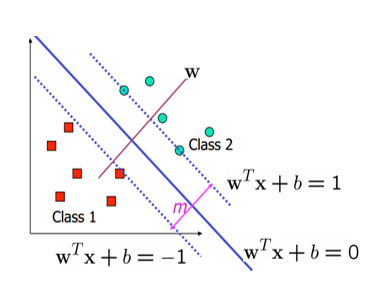
\includegraphics[width=0.6\linewidth]{5.png}
\end{figure}

\subsection{Matlab代码}
\begin{lstlisting}[language=matlab]
	data = load("./data5/training_2.txt");
	pos = [];
	neg = [];
	[m, n] = size(data);
	m = 100;
	
	for i = 1 : m
		if data(i, n) == 1
			pos = [pos; data(i, 1 : n - 1)];
		else
			neg = [neg; data(i, 1 : n - 1)];
		end
	end
	
	plot(pos(:, 1), pos(:, 2), '+');
	hold on;
	plot(neg(:, 1), neg(:, 2), 'o');
	
	prob = optimproblem('ObjectiveSense', 'max');
	 
	
	X = data(1 : m, 1 : n - 1);
	Y = data(1 : m, n);
	clear data;
	
	alpha = optimvar("alpha", size(X, 1), 1, 'LowerBound', 0);
	tmp = (Y * Y') .* (X * X') .* (alpha * alpha');
	prob.Objective = sum(alpha) - 0.5 * sum(sum(tmp));
	prob.Constraints.con = sum(alpha .* Y) == 0;
	
	[s, f] = solve(prob);
	
	w = zeros(1, n - 1);
	for i = 1 : size(X, 1)
		w = w + s.alpha(i) * Y(i) * X(i, :);
	end
	
	ys = 0;
	xs = zeros(1, n - 1);
	for i = 1 : size(X, 1)
		if (s.alpha(i) > 1e-6)
			ys = Y(i);
			xs = X(i, :);
			break;
		end
	end
	
	b = ys;
	for i = 1 : size(X, 1)
		b = b - s.alpha(i) * Y(i) * X(i, :) * xs';
	end
	
	xs = 20 : 1 : 180;
	ys = (-w(1) * xs - b) / w(2);
	plot(xs, ys, 'b-');
	ys = (1 - w(1) * xs - b) / w(2);
	plot(xs, ys, 'k--');
	ys = (-1 - w(1) * xs - b) / w(2);
	plot(xs, ys, 'k--');
	title('training data 2');
	
	test_set = load("./data5/test_2.txt");
	pred = sign(test_set(:, 1 : 2) * w' + b);
	acc = sum(pred == test_set(:, 3)) / size(test_set, 1)
	% training data 1 acc = 99.6
	% training data 2 acc = 99.6
\end{lstlisting}

\subsection{运行结果}
\begin{figure}[H]
	\centering
	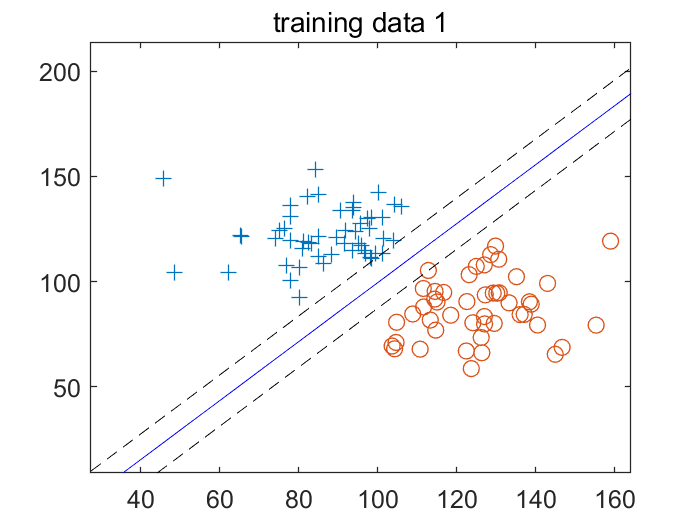
\includegraphics[width=0.6\linewidth]{1.png}
\end{figure}
\begin{figure}[H]
	\centering
	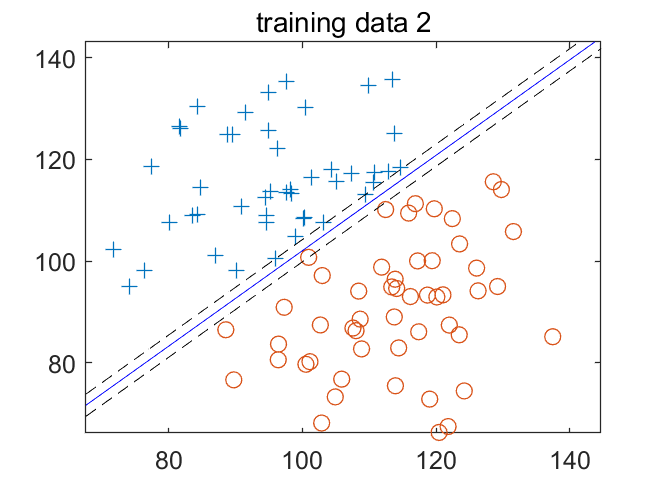
\includegraphics[width=0.6\linewidth]{2.png}
\end{figure}

在测试集上测试通过率均为99.6\%,即498/500。

\section{手写数字识别}
首先可以用给顶的strimage.m函数进行load数据:
\begin{figure}[H]
	\centering
	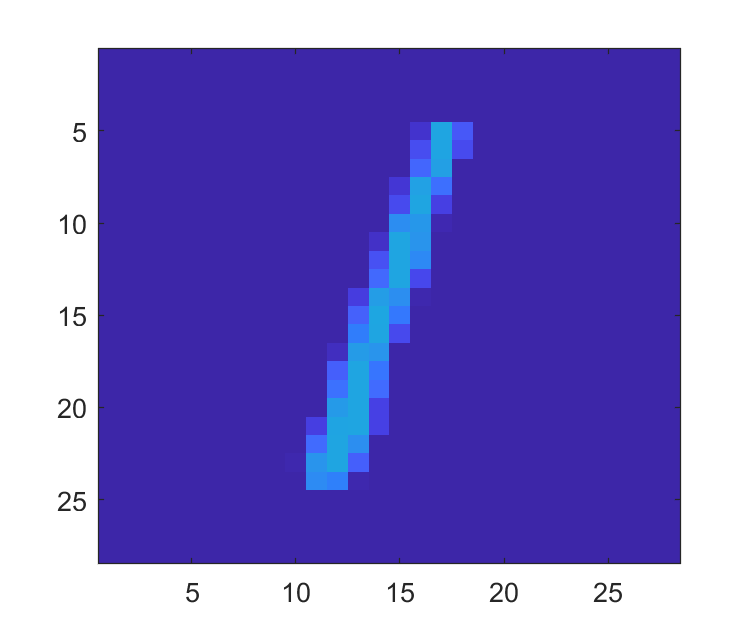
\includegraphics[width=0.4\linewidth]{6.png}
\end{figure}

然后求解策略就是用Linear SVM求解。实验文档要求增加如下约束条件来regularization:
\begin{equation}
	\alpha\leq C
\end{equation}

测试代码如下:
\begin{lstlisting}[language=matlab]
	[Y, X] = strimage(100);

	[m, n] = size(X);
	
	prob = optimproblem('ObjectiveSense', 'max');
	alpha = optimvar("alpha", size(X, 1), 1, 'LowerBound', 0);
	tmp = (Y * Y') .* (X * X') .* (alpha * alpha');
	prob.Objective = sum(alpha) - 0.5 * sum(sum(tmp));
	prob.Constraints.con = sum(alpha .* Y) == 0;
	
	prob.Constraints.con1 = alpha <= 10;
	
	[s, f] = solve(prob);
	
	w = zeros(1, n);
	for i = 1 : size(X, 1)
		w = w + s.alpha(i) * Y(i) * X(i, :);
	end
	
	ys = 0;
	xs = zeros(1, n);
	for i = 1 : size(X, 1)
		if (s.alpha(i) > 1e-6)
			ys = Y(i);
			xs = X(i, :);
			break;
		end
	end
	
	b = ys;
	for i = 1 : size(X, 1)
		b = b - s.alpha(i) * Y(i) * X(i, :) * xs';
	end
	
	[test_label, test_set] = strimage_test(1500);
	pred = sign(test_set(:, 1 : n) * w' + b);
	acc = sum(pred == test_label) / 1500
	% C = 0, 99.67%
	% C = 1, 99.8%
	% C = 2, 99.8%
	% C = 3, 99.8%
	% C = 10, 99.8%	
\end{lstlisting}

根据我的测试结果,选$C=1,2,3,10$均有着99.8\%的准确率。

\section{Nonlinear SVM}

当数据集线性不可分的情况,可以考虑使用\textbf{核函数},即对每个数据点$\textbf{x}_i$,构造一个新的特征值$\phi(\textbf{x}_i)$,使得数据集重新变得线性可分,是一个升维度的思想。
譬如若二维数据集$(x,y)$是$x^2+y^2\leq 1$的为类-1,若$x^2+y^2> 2$的为类+1,则它显然线性不可分,分界线是一个圆。但如果我增加特征值$z=\phi(x,y)=x^2+y^2$,那么数据集$(x,y,z)$就重现变得线性可分了,
分界平面为$z=1.5$。一张图说明数据转换过程:
\begin{figure}[H]
	\centering
	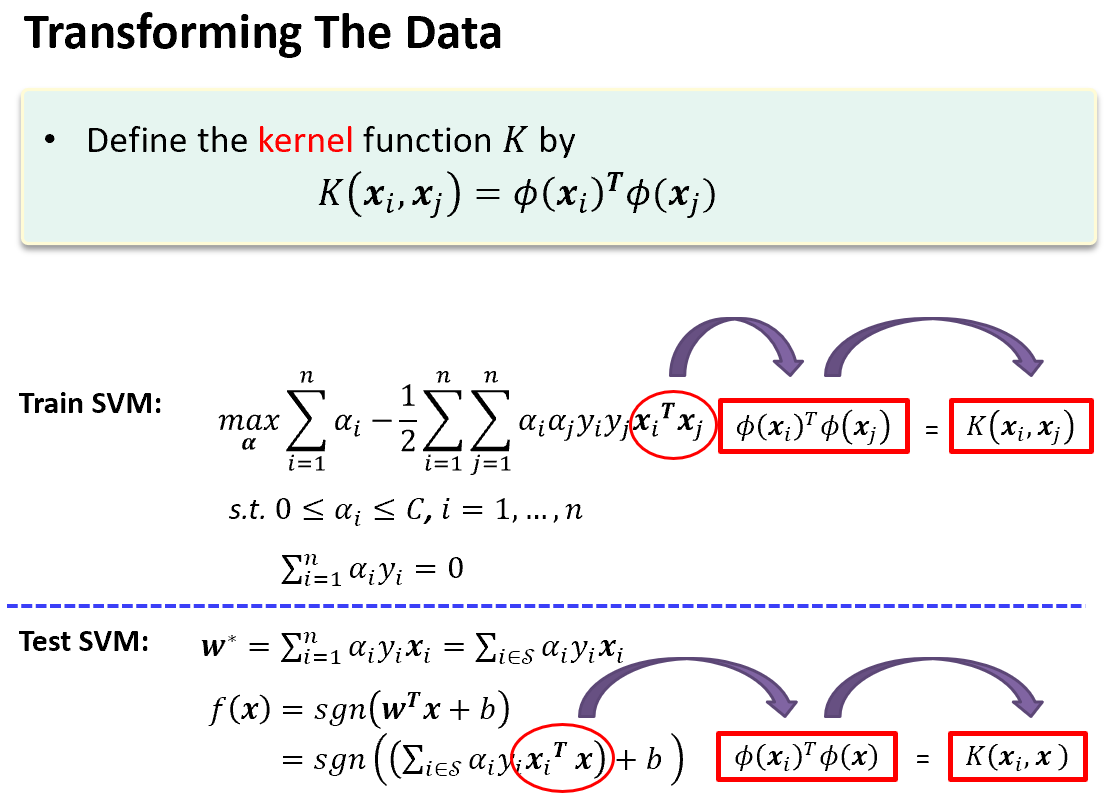
\includegraphics[width=\linewidth]{7.png}
\end{figure}

实验文档要求我们选择核函数为:
\begin{equation}
	K(\textbf{x}_i,\textbf{x}_j)=exp(-100\times||\textbf{x}_i-\textbf{x}_j||^2)
\end{equation}

之后就类似前面的一样训练和测试了。代码如下:
\begin{lstlisting}[language=matlab]
	data = load("./data5/training_3.txt");

	X = data(:, 1 : 2);
	Y = data(:, 3);
	xplot = linspace(min(X(:, 1)), max(X(:, 1)), 100)';
	yplot = linspace(min(X(:, 2)), max(X(:, 2)), 100)';
	[Xs, Ys] = meshgrid(xplot, yplot);

	prob = optimproblem('ObjectiveSense', 'max');
	alpha = optimvar("alpha", size(X, 1), 1, 'LowerBound', 0);

	K = zeros(size(X, 1), size(X, 1));
	for i = 1 : size(X, 1)
		for j = 1 : size(X, 1)
			K(i, j) = exp(-100 * norm(X(i, :) - X(j, :))^2);
		end
	end
	tmp = (Y * Y') .* (alpha * alpha') .* K;
	prob.Objective = sum(alpha) - 0.5 * sum(sum(tmp));
	prob.Constraints.con = sum(alpha .* Y) == 0;

	[s, f] = solve(prob);

	ys = 0;
	xs = zeros(1, 2);
	for i = 1 : size(X, 1)
		if (s.alpha(i) > 1e-6)
			ys = Y(i);
			xs = X(i, :);
			break;
		end
	end

	b = ys;
	for i = 1 : size(X, 1)
		b = b - s.alpha(i) * Y(i) * X(i, :) * xs';
	end

	vals = zeros(size(xplot, 1), size(yplot, 1));
	for i = 1 : 100
		for j = 1 : 100
			x = [xplot(i); yplot(j)];
			vals(i, j) = b;
			for k = 1 : size(X, 1)
				vals(i, j) = vals(i, j) + s.alpha(k) * Y(k) * exp(-100 * norm(X(k, :) - x)^2);
			end
		end
	end

	pos = [];
	neg = [];
	for i = 1 : size(X, 1)
		if (Y(i) == 1)
			pos = [pos; X(i, :)];
		else
			neg = [neg; X(i, :)];
		end
	end
	plot(pos(:, 1), pos(:, 2), 'r+', neg(:, 1), neg(:, 2), 'bo');
	hold on;
	colormap bone
	contour(Xs, Ys, vals, -20 : 0.1 : 0);
	title('Non Linear training 3');
\end{lstlisting}

然后画出来的图如下:
\begin{figure}[H]
	\centering
	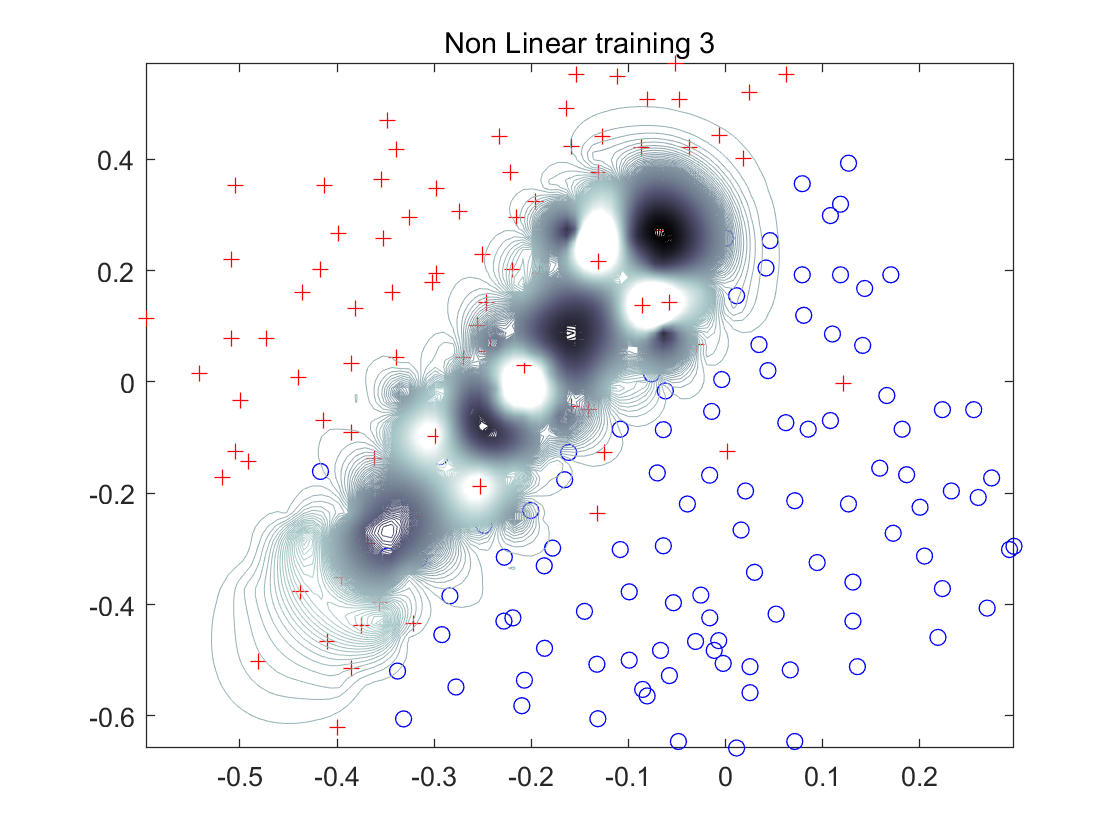
\includegraphics[width=\linewidth]{3.png}
\end{figure}

等高线圈起来的我画的是值为-20到0的范围。可以看到这些等高线在分界处很好地把-1类的数据点圈进去了,然后把+1类点丢在外面。

\end{document}